\documentclass[11pt]{article}
\usepackage{mathblatt}
% gesetzt von werkzeuge/setzer.py (Sorte selbst) aus dem Lernweg L75
% und den Bankzeilen; Muster bau/proben/2026-10-09/hypotenuse-muster.
\usepackage{enumitem}
\usepackage{adjustbox,varwidth}
\newgeometry{a4paper,margin=18mm,top=15mm,bottom=20mm,footskip=9mm}
\pagestyle{fancy}\fancyhf{}\renewcommand{\headrulewidth}{0pt}
\fancyfoot[L]{\footnotesize\color{mbgrau}L75 \textperiodcentered{} Körper erkennen, Netze, Schrägbilder}
\fancyfoot[R]{\footnotesize\color{mbgrau}\thepage}
\setlength{\parskip}{3pt}
\renewcommand{\kreuz}[1]{\mbox{$\square$\ #1}\quad}
\newcommand{\kreuzl}[1]{\par\hangindent1.4em\hangafter1\noindent$\square$\ #1}
\newcommand{\aufg}[3]{\par\noindent\makebox[0pt][r]{#3}\begin{minipage}[t]{\linewidth}#1\end{minipage}\par}
\newcommand{\aufgg}[4]{\par\noindent\makebox[0pt][r]{#4}\begin{minipage}[t]{0.6\linewidth}\vspace{0pt}#1\end{minipage}\hfill
  \begin{minipage}[t]{0.37\linewidth}\vspace{0pt}\centering #2\end{minipage}\par}
\newcommand{\nr}[1]{\makebox[7mm][l]{\textbf{#1}}}
\newcommand{\lsg}[3]{\par\noindent\begin{minipage}[t]{9mm}\textbf{#1}\end{minipage}%
  \begin{minipage}[t]{52mm}\raggedright\bfseries\boldmath #2\end{minipage}\hspace{3mm}%
  \begin{minipage}[t]{\dimexpr\linewidth-64mm\relax}\raggedright\small #3\end{minipage}\par\vspace{4pt}}
\newlength{\kr}
\makeatletter
\newcommand{\karomerk}[2]{\protected@write\@auxout{}{\string\karoseite{#1}{#2}{\thepage}}}
\newcommand{\karoseite}[3]{\expandafter\xdef\csname karo@#1@#2\endcsname{#3}}
\newcommand{\karohinweis}[3]{\karomerk{h}{#1}\ifcsname karo@k@#1\endcsname
  \ifnum\csname karo@k@#1\endcsname=0\csname karo@h@#1\endcsname\relax#2\else#3\fi
  \else#3\fi}
\makeatother
\begin{document}

\noindent{\LARGE\bfseries Körper erkennen, Netze, Schrägbilder}\par\smallskip
\noindent{\small\color{mbgrau}Selbstlernheft Klasse 6 \textperiodcentered{} mit Lösungsheft \textperiodcentered{} Kennung L75}\par\medskip
\noindent\textbf{So nutzt du das Heft:} Lies im Abschnitt das Beispiel. Rechne dann die Aufgaben der Reihe nach und vergleiche jede sofort mit dem Lösungsheft. Kreuze „kann ich“ an, wenn du die letzte Aufgabe (\emph{Ziel}) allein schaffst.\par
\noindent Mehr Aufgaben zu einem Abschnitt: Kennung deinem Nachhilfelehrer schicken (z.\,B. „L75 mehr B“).\par\medskip
{\arrayrulecolor{mbgrau}\renewcommand{\arraystretch}{1.3}
\noindent\begin{tabular}{|>{\bfseries}p{10mm}|p{112mm}|>{\raggedleft\arraybackslash}p{10mm}|>{\centering\arraybackslash}p{14mm}|}\hline
\rowcolor{black!8} & \textbf{Abschnitt} & \textbf{Seite} & \textbf{kann ich}\\\hline
A & Körper erkennen und zählen & \pageref{s:A} & $\square$\\\hline
B & Würfelnetze: was liegt gegenüber? & \pageref{s:B} & $\square$\\\hline
C & Netze von Quader und anderen Körpern & \pageref{s:C} & $\square$\\\hline
D & Schrägbilder & \pageref{s:D} & $\square$\\\hline
T & Probetest & \pageref{s:T} & $\square$\\\hline
\end{tabular}}\par\bigskip

\begin{tcolorbox}[colback=mbkasten,colframe=mbgrau,boxrule=0.5pt,arc=1mm,left=3mm,right=3mm,top=2mm,bottom=2mm,title={\bfseries Formel auf einen Blick},coltitle=black,colbacktitle=black!10]
{\Large Grundfläche mit $n$ Ecken:\par Prisma: Ecken $n + n$, Kanten $n + n + n$, Flächen $2 + n$\par Pyramide: Ecken $n + 1$, Kanten $n + n$, Flächen $1 + n$}\par\medskip
In Worten: Ein Netz ist der aufgeklappte Körper, ein Schrägbild der Körper auf Kästchen gezeichnet.\par\medskip
\end{tcolorbox}
\medskip\noindent\textbf{Typische Fehler – so nicht}\par\smallskip
\noindent\nr{$\times$}Ecken und Kanten verwechselt. Ecken sind Punkte, Kanten sind Linien.\par
\noindent\nr{$\times$}Im Würfelnetz die Nachbarfläche als Gegenfläche genommen.\par
\noindent\nr{$\times$}Im Schrägbild die Tiefe in voller Länge gezeichnet.\par
\clearpage\label{s:A}\noindent\colorbox{black!12}{\makebox[10mm]{\Large\bfseries\strut A}}\hspace{3mm}{\Large\bfseries Körper erkennen und zählen}\par\smallskip
\noindent Ein \textbf{Prisma} hat zwei gleiche Flächen, die sich gegenüberliegen (Grund- und Deckfläche), dazwischen Rechtecke; Quader und Würfel sind Prismen. Eine \textbf{Pyramide} hat eine Grundfläche und Dreiecke, die sich in der Spitze treffen; Zylinder, Kegel und Kugel haben gekrümmte Flächen.\par\medskip
\noindent\textbf{Formel}\par\nopagebreak\noindent\hspace*{4mm}\begin{minipage}{\dimexpr\linewidth-4mm\relax}Prisma: Kanten $n + n + n$ \qquad Pyramide: Kanten $n + n$ \qquad {\small ($n$ Ecken der Grundfläche)}\end{minipage}\par\medskip
\noindent\textbf{Beispiel}\quad Ein Zelt hat die Form im Bild. Es soll als Kantenmodell aus Stäben und Knetkugeln gebaut werden. Wie heißt der Körper? Wie viele Stäbe und wie viele Kugeln braucht man? Wie viele Flächen hat er?\par\smallskip
\noindent\begin{minipage}[t]{0.6\linewidth}\vspace{0pt}\par\noindent\hangindent6mm\hangafter1\makebox[6mm][l]{\textbf{1}}Vorn und hinten ist je ein gleiches Dreieck, dazwischen sind Rechtecke: ein \textbf{Dreiecksprisma}. Es liegt auf einem Rechteck.\par\smallskip\par\noindent\hangindent6mm\hangafter1\makebox[6mm][l]{\textbf{2}}Kugeln = Ecken: vorn $3$, hinten $3$, also $3 + 3 = 6$.\par\smallskip\par\noindent\hangindent6mm\hangafter1\makebox[6mm][l]{\textbf{3}}Stäbe = Kanten: vorn $3$, hinten $3$, von vorn nach hinten $3$, also $3 + 3 + 3 = 9$.\par\smallskip\par\noindent\hangindent6mm\hangafter1\makebox[6mm][l]{\textbf{4}}Flächen: $2$ Dreiecke und $3$ Rechtecke, also $5$.\par\smallskip\end{minipage}\hfill
\begin{minipage}[t]{0.37\linewidth}\vspace{0pt}\centering 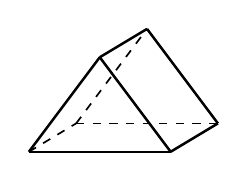
\begin{tikzpicture}[scale=0.6,font=\small,line join=round]\draw[line width=0.9pt] (0,0) -- (3,0);\draw[line width=0.9pt] (3,0) -- (1.5,2);\draw[line width=0.9pt] (0,0) -- (1.5,2);\draw[dashed,line width=0.6pt] (1,0.6) -- (4,0.6);\draw[line width=0.9pt] (4,0.6) -- (2.5,2.6);\draw[dashed,line width=0.6pt] (1,0.6) -- (2.5,2.6);\draw[line width=0.9pt] (3,0) -- (4,0.6);\draw[dashed,line width=0.6pt] (0,0) -- (1,0.6);\draw[line width=0.9pt] (1.5,2) -- (2.5,2.6);\end{tikzpicture}\end{minipage}\par\medskip
\noindent\textbf{Aufgaben}\hspace{1em}{\small\color{mbgrau}\karohinweis{A}{Rechne unten im Karo.}{Rechne auf einem extra Blatt.} Vergleiche jede Aufgabe gleich mit dem Lösungsheft.}\par\smallskip
\aufgg{\hangindent7mm\hangafter1\nr{1.}Wie heißen die vier Körper im Bild?}{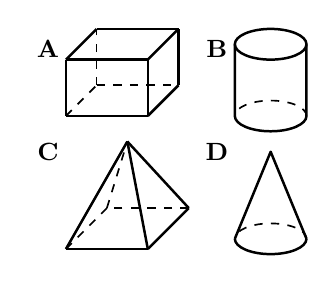
\begin{tikzpicture}[scale=0.65,font=\small,line join=round]\begin{scope}[shift={(0,2.6)}]\draw[line width=0.9pt] (0,0) -- (1.6,0);\draw[line width=0.9pt] (1.6,0) -- (1.6,1.1);\draw[line width=0.9pt] (1.6,1.1) -- (0,1.1);\draw[line width=0.9pt] (0,0) -- (0,1.1);\draw[dashed,line width=0.6pt] (0.6,0.6) -- (2.2,0.6);\draw[line width=0.9pt] (2.2,0.6) -- (2.2,1.7);\draw[line width=0.9pt] (2.2,1.7) -- (0.6,1.7);\draw[dashed,line width=0.6pt] (0.6,0.6) -- (0.6,1.7);\draw[line width=0.9pt] (1.6,0) -- (2.2,0.6);\draw[dashed,line width=0.6pt] (0,0) -- (0.6,0.6);\draw[line width=0.9pt] (1.6,1.1) -- (2.2,1.7);\draw[line width=0.9pt] (0,1.1) -- (0.6,1.7);\end{scope}\node[font=\small\bfseries] at (-0.35,3.9) {A};\draw[line width=0.9pt] (3.3,4) -- (3.3,2.6) arc (180:360:0.7 and 0.3) -- (4.7,4);\draw[dashed,line width=0.6pt] (4.7,2.6) arc (0:180:0.7 and 0.3);\draw[line width=0.9pt] (4,4) ellipse (0.7 and 0.3);\node[font=\small\bfseries] at (2.95,3.9) {B};\begin{scope}[shift={(0,0)}]\draw[line width=0.9pt] (0,0) -- (1.6,0);\draw[line width=0.9pt] (1.6,0) -- (2.4,0.8);\draw[dashed,line width=0.6pt] (2.4,0.8) -- (0.8,0.8);\draw[dashed,line width=0.6pt] (0,0) -- (0.8,0.8);\draw[line width=0.9pt] (1.6,0) -- (1.2,2.1);\draw[line width=0.9pt] (0,0) -- (1.2,2.1);\draw[line width=0.9pt] (2.4,0.8) -- (1.2,2.1);\draw[dashed,line width=0.6pt] (0.8,0.8) -- (1.2,2.1);\end{scope}\node[font=\small\bfseries] at (-0.35,1.9) {C};\draw[line width=0.9pt] (3.3,0.2) -- (4,1.9) -- (4.7,0.2);\draw[line width=0.9pt] (3.3,0.2) arc (180:360:0.7 and 0.3);\draw[dashed,line width=0.6pt] (4.7,0.2) arc (0:180:0.7 and 0.3);\node[font=\small\bfseries] at (2.95,1.9) {D};\end{tikzpicture}}{}{}
\medskip
\aufgg{\hangindent7mm\hangafter1\nr{2.}Ein Turmdach hat die Form im Bild: eine Pyramide mit quadratischer Grundfläche. Wie viele Ecken, Kanten und Flächen hat sie?}{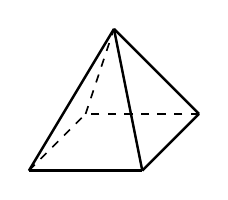
\begin{tikzpicture}[scale=0.6,font=\small,line join=round]\draw[line width=0.9pt] (0,0) -- (2.4,0);\draw[line width=0.9pt] (2.4,0) -- (3.6,1.2);\draw[dashed,line width=0.6pt] (3.6,1.2) -- (1.2,1.2);\draw[dashed,line width=0.6pt] (0,0) -- (1.2,1.2);\draw[line width=0.9pt] (2.4,0) -- (1.8,3);\draw[line width=0.9pt] (0,0) -- (1.8,3);\draw[line width=0.9pt] (3.6,1.2) -- (1.8,3);\draw[dashed,line width=0.6pt] (1.2,1.2) -- (1.8,3);\end{tikzpicture}}{}{}
\medskip
\aufgg{\hangindent7mm\hangafter1\nr{3.}Das Bild zeigt ein Stück von einem ungespitzten Bleistift. Wie heißt der Körper genau? Wie viele Ecken, Kanten und Flächen hat er?}{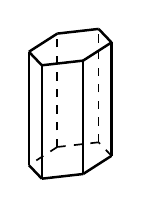
\begin{tikzpicture}[scale=0.6,font=\small,line join=round]\draw[dashed,line width=0.6pt] (2.074,0.499) -- (1.801,0.785);\draw[dashed,line width=0.6pt] (1.801,0.785) -- (0.927,0.686);\draw[dashed,line width=0.6pt] (0.927,0.686) -- (0.326,0.301);\draw[line width=0.9pt] (0.326,0.301) -- (0.599,0.015);\draw[line width=0.9pt] (0.599,0.015) -- (1.473,0.114);\draw[line width=0.9pt] (2.074,0.499) -- (1.473,0.114);\draw[line width=0.9pt] (2.074,2.899) -- (1.801,3.185);\draw[line width=0.9pt] (1.801,3.185) -- (0.927,3.086);\draw[line width=0.9pt] (0.927,3.086) -- (0.326,2.701);\draw[line width=0.9pt] (0.326,2.701) -- (0.599,2.415);\draw[line width=0.9pt] (0.599,2.415) -- (1.473,2.514);\draw[line width=0.9pt] (2.074,2.899) -- (1.473,2.514);\draw[dashed,line width=0.6pt] (1.801,0.785) -- (1.801,3.185);\draw[line width=0.9pt] (2.074,0.499) -- (2.074,2.899);\draw[dashed,line width=0.6pt] (0.927,0.686) -- (0.927,3.086);\draw[line width=0.9pt] (0.326,0.301) -- (0.326,2.701);\draw[line width=0.9pt] (0.599,0.015) -- (0.599,2.415);\draw[line width=0.9pt] (1.473,0.114) -- (1.473,2.514);\end{tikzpicture}}{}{}
\medskip
\aufg{\hangindent7mm\hangafter1\nr{4.}Ein Pavillondach hat die Form einer Pyramide mit sechseckiger Grundfläche. Tim baut ein Kantenmodell davon. Er hat $10$ Stäbe und $8$ Knetkugeln. Reicht das? Wie viele Stäbe oder Kugeln fehlen oder bleiben übrig?}{}{{\scriptsize\color{mbgrau}Ziel\hspace{2mm}}}
\medskip
\par\vspace{3mm}\setlength{\kr}{\dimexpr\pagegoal-\pagetotal-10mm\relax}%
\ifdim\kr>12mm\karomerk{k}{A}\noindent{\scriptsize\color{mbgrau}Platz zum Rechnen}\par\nointerlineskip\vspace{1mm}\noindent
\begin{tikzpicture}\clip (0,0) rectangle ({\linewidth-0.5mm},\kr);\draw[black!16,line width=0.3pt,step=5mm] (0,0) grid (\linewidth,\kr);\end{tikzpicture}\fi\par
\clearpage\label{s:B}\noindent\colorbox{black!12}{\makebox[10mm]{\Large\bfseries\strut B}}\hspace{3mm}{\Large\bfseries Würfelnetze: was liegt gegenüber?}\par\smallskip
\noindent Ein Würfelnetz besteht aus sechs Quadraten. In einer Reihe (waagerecht oder senkrecht) liegen sich zwei Flächen gegenüber, wenn genau eine Fläche dazwischen liegt.\par\medskip
\noindent\textbf{Formel}\par\nopagebreak\noindent\hspace*{4mm}\begin{minipage}{\dimexpr\linewidth-4mm\relax}\fbox{\strut A}\fbox{\strut B}\fbox{\strut C} \quad $\Rightarrow$ \quad A liegt C gegenüber.\end{minipage}\par\medskip
\noindent\textbf{Beispiel}\quad Vier Quadrate B, C, D, E liegen in einer Reihe. Oben an B hängt A, unten an D hängt F. Welche Flächen liegen sich gegenüber, wenn man daraus einen Würfel faltet?\par\smallskip
\noindent\begin{minipage}[t]{0.6\linewidth}\vspace{0pt}\par\noindent\hangindent6mm\hangafter1\makebox[6mm][l]{\textbf{1}}Skizziere das Netz (Bild).\par\smallskip\par\noindent\hangindent6mm\hangafter1\makebox[6mm][l]{\textbf{2}}In der Reihe B C D E: Zwischen B und D liegt genau C, also liegen B und D gegenüber. Zwischen C und E liegt D: C und E gegenüber.\par\smallskip\par\noindent\hangindent6mm\hangafter1\makebox[6mm][l]{\textbf{3}}Übrig sind A und F. Sie berühren sich nicht, also liegen sie gegenüber.\par\smallskip\par\noindent\hangindent6mm\hangafter1\makebox[6mm][l]{\textbf{4}}Jede Fläche hat genau eine Gegenfläche: Es ist ein Würfelnetz.\par\smallskip\end{minipage}\hfill
\begin{minipage}[t]{0.37\linewidth}\vspace{0pt}\centering 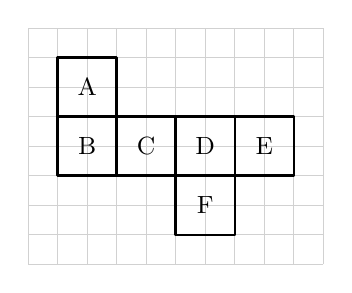
\begin{tikzpicture}[scale=0.75,font=\small,line join=round]\draw[black!18,line width=0.3pt,step=0.5] (-0.5,-0.5) grid (4.5,3.5);\draw[line width=0.9pt] (0,2) rectangle (1,3);\node at (0.5,2.5) {A};\draw[line width=0.9pt] (0,1) rectangle (1,2);\node at (0.5,1.5) {B};\draw[line width=0.9pt] (1,1) rectangle (2,2);\node at (1.5,1.5) {C};\draw[line width=0.9pt] (2,1) rectangle (3,2);\node at (2.5,1.5) {D};\draw[line width=0.9pt] (3,1) rectangle (4,2);\node at (3.5,1.5) {E};\draw[line width=0.9pt] (2,0) rectangle (3,1);\node at (2.5,0.5) {F};\end{tikzpicture}\end{minipage}\par\medskip
\noindent\textbf{Aufgaben}\hspace{1em}{\small\color{mbgrau}\karohinweis{B}{Rechne unten im Karo.}{Rechne auf einem extra Blatt.} Vergleiche jede Aufgabe gleich mit dem Lösungsheft.}\par\smallskip
\aufgg{\hangindent7mm\hangafter1\nr{1.}Aus dem Netz im Bild wird ein Würfel gefaltet. Schreib die drei Paare von Flächen auf, die sich gegenüberliegen.}{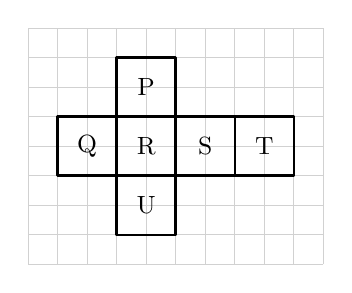
\begin{tikzpicture}[scale=0.75,font=\small,line join=round]\draw[black!18,line width=0.3pt,step=0.5] (-0.5,-0.5) grid (4.5,3.5);\draw[line width=0.9pt] (1,2) rectangle (2,3);\node at (1.5,2.5) {P};\draw[line width=0.9pt] (0,1) rectangle (1,2);\node at (0.5,1.5) {Q};\draw[line width=0.9pt] (1,1) rectangle (2,2);\node at (1.5,1.5) {R};\draw[line width=0.9pt] (2,1) rectangle (3,2);\node at (2.5,1.5) {S};\draw[line width=0.9pt] (3,1) rectangle (4,2);\node at (3.5,1.5) {T};\draw[line width=0.9pt] (1,0) rectangle (2,1);\node at (1.5,0.5) {U};\end{tikzpicture}}{}{}
\medskip
\aufgg{\hangindent7mm\hangafter1\nr{2.}Kann man aus dem Netz im Bild einen Würfel falten? Begründe mit den Gegenflächen.}{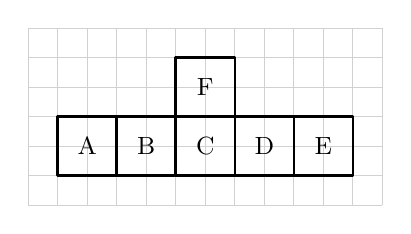
\begin{tikzpicture}[scale=0.75,font=\small,line join=round]\draw[black!18,line width=0.3pt,step=0.5] (-0.5,-0.5) grid (5.5,2.5);\draw[line width=0.9pt] (2,1) rectangle (3,2);\node at (2.5,1.5) {F};\draw[line width=0.9pt] (0,0) rectangle (1,1);\node at (0.5,0.5) {A};\draw[line width=0.9pt] (1,0) rectangle (2,1);\node at (1.5,0.5) {B};\draw[line width=0.9pt] (2,0) rectangle (3,1);\node at (2.5,0.5) {C};\draw[line width=0.9pt] (3,0) rectangle (4,1);\node at (3.5,0.5) {D};\draw[line width=0.9pt] (4,0) rectangle (5,1);\node at (4.5,0.5) {E};\end{tikzpicture}}{}{}
\medskip
\aufgg{\hangindent7mm\hangafter1\nr{3.}Aus dem Netz wird ein Spielwürfel. Gegenüberliegende Augenzahlen ergeben zusammen $7$. Welche Zahlen gehören auf X, Y und Z?}{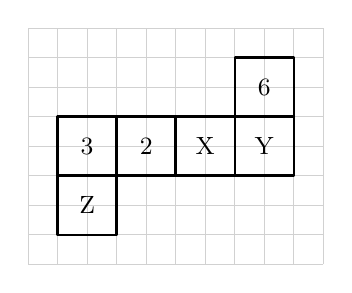
\begin{tikzpicture}[scale=0.75,font=\small,line join=round]\draw[black!18,line width=0.3pt,step=0.5] (-0.5,-0.5) grid (4.5,3.5);\draw[line width=0.9pt] (3,2) rectangle (4,3);\node at (3.5,2.5) {6};\draw[line width=0.9pt] (0,1) rectangle (1,2);\node at (0.5,1.5) {3};\draw[line width=0.9pt] (1,1) rectangle (2,2);\node at (1.5,1.5) {2};\draw[line width=0.9pt] (2,1) rectangle (3,2);\node at (2.5,1.5) {X};\draw[line width=0.9pt] (3,1) rectangle (4,2);\node at (3.5,1.5) {Y};\draw[line width=0.9pt] (0,0) rectangle (1,1);\node at (0.5,0.5) {Z};\end{tikzpicture}}{}{}
\medskip
\aufgg{\hangindent7mm\hangafter1\nr{4.}Mia bastelt einen Spielwürfel. Ihr Netz: vier Quadrate in einer Reihe mit $1$, $2$, $6$, $3$. Oben an der $2$ hängt die $5$, unten an der $3$ hängt die $4$. Auf einem Spielwürfel ergeben gegenüberliegende Zahlen $7$. Stimmt Mias Würfel? Wenn nicht: Welche zwei Zahlen kann sie tauschen? Finde eine Möglichkeit. Skizziere zuerst.}{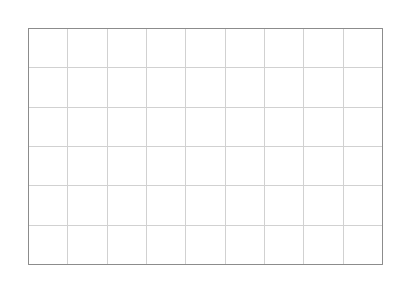
\begin{tikzpicture}[scale=1,font=\small,line join=round]\draw[black!18,line width=0.3pt,step=0.5] (0,0) grid (4.5,3);\draw[black!45,line width=0.4pt] (0,0) rectangle (4.5,3);\end{tikzpicture}}{}{{\scriptsize\color{mbgrau}Ziel\hspace{2mm}}}
\medskip
\par\vspace{3mm}\setlength{\kr}{\dimexpr\pagegoal-\pagetotal-10mm\relax}%
\ifdim\kr>12mm\karomerk{k}{B}\noindent{\scriptsize\color{mbgrau}Platz zum Rechnen}\par\nointerlineskip\vspace{1mm}\noindent
\begin{tikzpicture}\clip (0,0) rectangle ({\linewidth-0.5mm},\kr);\draw[black!16,line width=0.3pt,step=5mm] (0,0) grid (\linewidth,\kr);\end{tikzpicture}\fi\par
\clearpage\label{s:C}\noindent\colorbox{black!12}{\makebox[10mm]{\Large\bfseries\strut C}}\hspace{3mm}{\Large\bfseries Netze von Quader und anderen Körpern}\par\smallskip
\noindent Ein Quader hat drei Paare gleicher Rechtecke: Boden und Deckel, vorn und hinten, die zwei Seiten. Am Netz erkennst du den Körper an den Formen seiner Flächen.\par\medskip
\noindent\textbf{Beispiel}\quad Eine Streichholzschachtel ist ein Quader: $3$\,cm lang, $2$\,cm breit, $1$\,cm hoch. Zeichne ihr Netz in wahrer Größe.\par\smallskip
\noindent\begin{minipage}[t]{0.6\linewidth}\vspace{0pt}\par\noindent\hangindent6mm\hangafter1\makebox[6mm][l]{\textbf{1}}Drei Paare Rechtecke: Boden und Deckel $3 \times 2$, vorn und hinten $3 \times 1$, Seiten $2 \times 1$ (in cm).\par\smallskip\par\noindent\hangindent6mm\hangafter1\makebox[6mm][l]{\textbf{2}}Streifen von unten nach oben: vorn, Boden, hinten, Deckel. $3$\,cm sind $6$ Kästchen.\par\smallskip\par\noindent\hangindent6mm\hangafter1\makebox[6mm][l]{\textbf{3}}Die Seiten links und rechts an den Boden.\par\smallskip\par\noindent\hangindent6mm\hangafter1\makebox[6mm][l]{\textbf{4}}Prüfen: Kanten, die beim Falten aufeinandertreffen, sind gleich lang.\par\smallskip\par\noindent\hangindent6mm\hangafter1\makebox[6mm][l]{\textbf{5}}Das Netz ist $1 + 3 + 1 = 5$\,cm breit und $1 + 2 + 1 + 2 = 6$\,cm hoch.\par\smallskip\end{minipage}\hfill
\begin{minipage}[t]{0.37\linewidth}\vspace{0pt}\centering 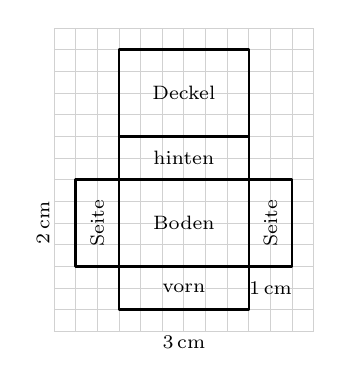
\begin{tikzpicture}[scale=0.55,font=\small,line join=round]\draw[black!18,line width=0.3pt,step=0.5] (-0.5,-0.5) grid (5.5,6.5);\draw[line width=0.9pt] (1,0) rectangle (4,1);\node[font=\scriptsize] at (2.5,0.5) {vorn};\draw[line width=0.9pt] (1,1) rectangle (4,3);\node[font=\scriptsize] at (2.5,2) {Boden};\draw[line width=0.9pt] (1,3) rectangle (4,4);\node[font=\scriptsize] at (2.5,3.5) {hinten};\draw[line width=0.9pt] (1,4) rectangle (4,6);\node[font=\scriptsize] at (2.5,5) {Deckel};\draw[line width=0.9pt] (0,1) rectangle (1,3);\draw[line width=0.9pt] (4,1) rectangle (5,3);\node[font=\scriptsize] at (2.5,-0.75) {3\,cm};\node[font=\scriptsize,rotate=90] at (-0.75,2) {2\,cm};\node[font=\scriptsize] at (4.5,0.5) {1\,cm};\node[font=\scriptsize,rotate=90] at (0.5,2) {Seite};\node[font=\scriptsize,rotate=90] at (4.5,2) {Seite};\end{tikzpicture}\end{minipage}\par\medskip
\noindent\textbf{Aufgaben}\hspace{1em}{\small\color{mbgrau}\karohinweis{C}{Rechne unten im Karo.}{Rechne auf einem extra Blatt.} Vergleiche jede Aufgabe gleich mit dem Lösungsheft.}\par\smallskip
\aufgg{\hangindent7mm\hangafter1\nr{1.}Welcher Körper entsteht aus jedem Netz im Bild?}{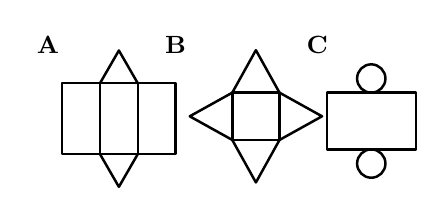
\begin{tikzpicture}[scale=0.6,font=\small,line join=round]\draw[line width=0.9pt] (0,0.7) rectangle (0.8,2.2);\draw[line width=0.9pt] (0.8,0.7) rectangle (1.6,2.2);\draw[line width=0.9pt] (1.6,0.7) rectangle (2.4,2.2);\draw[line width=0.9pt] (0.8,2.2) -- (1.2,2.893) -- (1.6,2.2);\draw[line width=0.9pt] (0.8,0.7) -- (1.2,0.007) -- (1.6,0.7);\node[font=\small\bfseries] at (-0.3,3) {A};\draw[line width=0.9pt] (3.6,1) rectangle (4.6,2);\draw[line width=0.9pt] (3.6,2) -- (4.1,2.9) -- (4.6,2);\draw[line width=0.9pt] (3.6,1) -- (4.1,0.1) -- (4.6,1);\draw[line width=0.9pt] (3.6,1) -- (2.7,1.5) -- (3.6,2);\draw[line width=0.9pt] (4.6,1) -- (5.5,1.5) -- (4.6,2);\node[font=\small\bfseries] at (2.4,3) {B};\draw[line width=0.9pt] (5.6,0.8) rectangle (7.485,2);\draw[line width=0.9pt] (6.542,2.3) circle (0.3);\draw[line width=0.9pt] (6.542,0.5) circle (0.3);\node[font=\small\bfseries] at (5.4,3) {C};\end{tikzpicture}}{}{}
\medskip
\aufgg{\hangindent7mm\hangafter1\nr{2.}Im Netz des Quaders fehlt ein Rechteck. Wie lang und wie breit ist es, und wo muss es hin?}{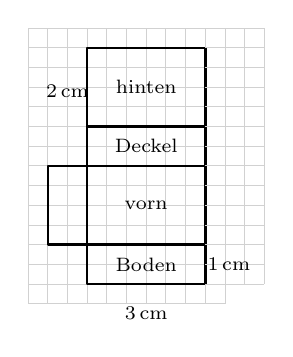
\begin{tikzpicture}[scale=0.5,font=\small,line join=round]\draw[black!18,line width=0.3pt,step=0.5] (-0.5,-0.5) grid (4.5,6.5);\draw[line width=0.9pt] (1,0) rectangle (4,1);\node[font=\scriptsize] at (2.5,0.5) {Boden};\draw[line width=0.9pt] (1,1) rectangle (4,3);\node[font=\scriptsize] at (2.5,2) {vorn};\draw[line width=0.9pt] (1,3) rectangle (4,4);\node[font=\scriptsize] at (2.5,3.5) {Deckel};\draw[line width=0.9pt] (1,4) rectangle (4,6);\node[font=\scriptsize] at (2.5,5) {hinten};\draw[line width=0.9pt] (0,1) rectangle (1,3);\draw[black!18,line width=0.3pt,step=0.5] (4,0) grid (5.5,6.5);\node[font=\scriptsize] at (2.5,-0.75) {3\,cm};\node[font=\scriptsize] at (4.6,0.5) {1\,cm};\node[font=\scriptsize] at (0.5,4.9) {2\,cm};\end{tikzpicture}}{}{}
\medskip
\aufgg{\hangindent7mm\hangafter1\nr{3.}Eine Packung Kaugummi ist ein Quader: $4$\,cm lang, $1$\,cm breit, $1$\,cm hoch. Zeichne ihr Netz in wahrer Größe in das Kästchenfeld.}{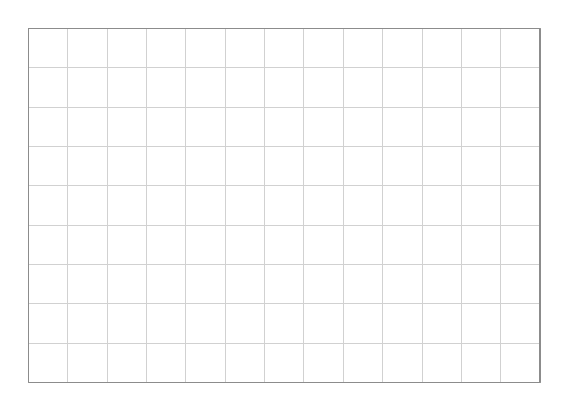
\begin{tikzpicture}[scale=1,font=\small,line join=round]\draw[black!18,line width=0.3pt,step=0.5] (0,0) grid (6.5,4.5);\draw[black!45,line width=0.4pt] (0,0) rectangle (6.5,4.5);\end{tikzpicture}}{}{}
\medskip
\aufgg{\hangindent7mm\hangafter1\nr{4.}Ben will eine Schachtel bauen: einen Quader, $6$\,cm lang, $4$\,cm breit und $2$\,cm hoch. Er hat ein Stück Karton, $12$\,cm $\times$ $12$\,cm. Skizziere ein Netz mit Maßen. Reicht der Karton?}{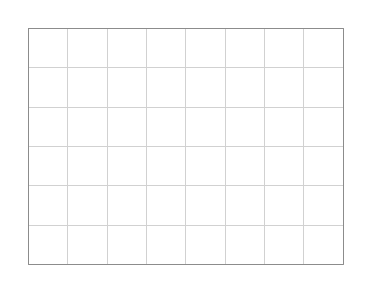
\begin{tikzpicture}[scale=1,font=\small,line join=round]\draw[black!18,line width=0.3pt,step=0.5] (0,0) grid (4,3);\draw[black!45,line width=0.4pt] (0,0) rectangle (4,3);\end{tikzpicture}}{}{{\scriptsize\color{mbgrau}Ziel\hspace{2mm}}}
\medskip
\par\vspace{3mm}\setlength{\kr}{\dimexpr\pagegoal-\pagetotal-10mm\relax}%
\ifdim\kr>12mm\karomerk{k}{C}\noindent{\scriptsize\color{mbgrau}Platz zum Rechnen}\par\nointerlineskip\vspace{1mm}\noindent
\begin{tikzpicture}\clip (0,0) rectangle ({\linewidth-0.5mm},\kr);\draw[black!16,line width=0.3pt,step=5mm] (0,0) grid (\linewidth,\kr);\end{tikzpicture}\fi\par
\clearpage\label{s:D}\noindent\colorbox{black!12}{\makebox[10mm]{\Large\bfseries\strut D}}\hspace{3mm}{\Large\bfseries Schrägbilder}\par\smallskip
\noindent Im Schrägbild zeichnest du die Vorderfläche in wahrer Größe. Kanten nach hinten gehen schräg und werden kürzer; verdeckte Kanten zeichnest du gestrichelt.\par\medskip
\noindent\textbf{Formel}\par\nopagebreak\noindent\hspace*{4mm}\begin{minipage}{\dimexpr\linewidth-4mm\relax}1\,cm $=$ 2 Kästchen \qquad je 1\,cm nach hinten: 1 Kästchendiagonale ($\tfrac12$\,cm nach rechts, $\tfrac12$\,cm nach oben)\end{minipage}\par\medskip
\noindent\textbf{Beispiel}\quad Ein Quader ist $3$\,cm lang, $2$\,cm tief und $2$\,cm hoch. Zeichne sein Schrägbild auf Kästchen.\par\smallskip
\noindent\begin{minipage}[t]{0.6\linewidth}\vspace{0pt}\par\noindent\hangindent6mm\hangafter1\makebox[6mm][l]{\textbf{1}}Vorderfläche in wahrer Größe: $3$\,cm $\times$ $2$\,cm, also $6 \times 4$ Kästchen.\par\smallskip\par\noindent\hangindent6mm\hangafter1\makebox[6mm][l]{\textbf{2}}Tiefe $2$\,cm: von den Ecken je $2$ Kästchendiagonalen nach rechts oben.\par\smallskip\par\noindent\hangindent6mm\hangafter1\makebox[6mm][l]{\textbf{3}}Hintere Ecken verbinden. Kanten, die man nicht sieht, gestrichelt (hier $3$).\par\smallskip\par\noindent\hangindent6mm\hangafter1\makebox[6mm][l]{\textbf{4}}Das Bild ist $3 + 1 = 4$\,cm breit und $2 + 1 = 3$\,cm hoch.\par\smallskip\par\noindent\hangindent6mm\hangafter1\makebox[6mm][l]{\textbf{5}}Die Körperhöhe ($2$\,cm) steht senkrecht. Bei einer Pyramide geht sie von der Spitze senkrecht zur Mitte der Grundfläche – sie ist keine Kante.\par\smallskip\end{minipage}\hfill
\begin{minipage}[t]{0.37\linewidth}\vspace{0pt}\centering 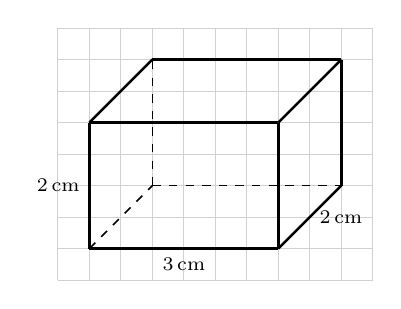
\begin{tikzpicture}[scale=0.8,font=\small,line join=round]\draw[black!18,line width=0.3pt,step=0.5] (-0.5,-0.5) grid (4.5,3.5);\draw[line width=0.9pt] (0,0) -- (3,0);\draw[line width=0.9pt] (3,0) -- (3,2);\draw[line width=0.9pt] (3,2) -- (0,2);\draw[line width=0.9pt] (0,0) -- (0,2);\draw[dashed,line width=0.6pt] (1,1) -- (4,1);\draw[line width=0.9pt] (4,1) -- (4,3);\draw[line width=0.9pt] (4,3) -- (1,3);\draw[dashed,line width=0.6pt] (1,1) -- (1,3);\draw[line width=0.9pt] (3,0) -- (4,1);\draw[dashed,line width=0.6pt] (0,0) -- (1,1);\draw[line width=0.9pt] (3,2) -- (4,3);\draw[line width=0.9pt] (0,2) -- (1,3);\node[font=\scriptsize,below] at (1.5,0) {3\,cm};\node[font=\scriptsize,left] at (0,1) {2\,cm};\node[font=\scriptsize,right] at (3.5,0.5) {2\,cm};\end{tikzpicture}\end{minipage}\par\medskip
\noindent\textbf{Aufgaben}\hspace{1em}{\small\color{mbgrau}\karohinweis{D}{Rechne unten im Karo.}{Rechne auf einem extra Blatt.} Vergleiche jede Aufgabe gleich mit dem Lösungsheft.}\par\smallskip
\aufgg{\hangindent7mm\hangafter1\nr{1.}Ein Würfel hat $3$\,cm Kantenlänge. Zeichne sein Schrägbild in das Kästchenfeld.}{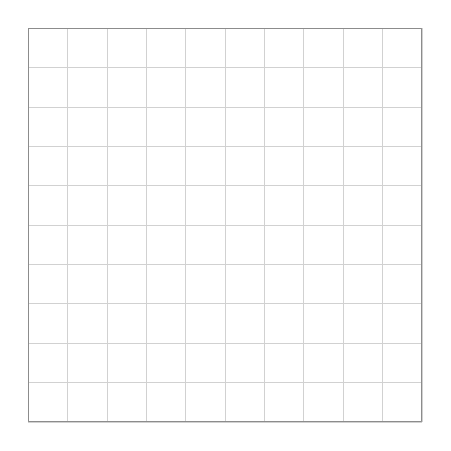
\begin{tikzpicture}[scale=1,font=\small,line join=round]\draw[black!18,line width=0.3pt,step=0.5] (0,0) grid (5,5);\draw[black!45,line width=0.4pt] (0,0) rectangle (5,5);\end{tikzpicture}}{}{}
\medskip
\aufgg{\hangindent7mm\hangafter1\nr{2.}Das Bild zeigt das Schrägbild eines Quaders (2 Kästchen $=$ 1\,cm). Wie lang, wie hoch und wie tief ist der Quader wirklich? Wie viele Kanten sind verdeckt?}{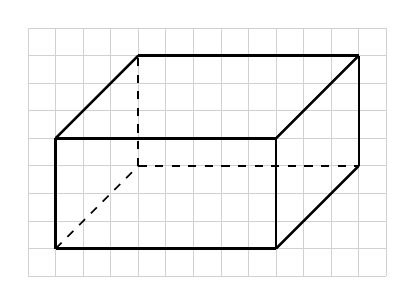
\begin{tikzpicture}[scale=0.7,font=\small,line join=round]\draw[black!18,line width=0.3pt,step=0.5] (-0.5,-0.5) grid (6,4);\draw[line width=0.9pt] (0,0) -- (4,0);\draw[line width=0.9pt] (4,0) -- (4,2);\draw[line width=0.9pt] (4,2) -- (0,2);\draw[line width=0.9pt] (0,0) -- (0,2);\draw[dashed,line width=0.6pt] (1.5,1.5) -- (5.5,1.5);\draw[line width=0.9pt] (5.5,1.5) -- (5.5,3.5);\draw[line width=0.9pt] (5.5,3.5) -- (1.5,3.5);\draw[dashed,line width=0.6pt] (1.5,1.5) -- (1.5,3.5);\draw[line width=0.9pt] (4,0) -- (5.5,1.5);\draw[dashed,line width=0.6pt] (0,0) -- (1.5,1.5);\draw[line width=0.9pt] (4,2) -- (5.5,3.5);\draw[line width=0.9pt] (0,2) -- (1.5,3.5);\end{tikzpicture}}{}{}
\medskip
\aufgg{\hangindent7mm\hangafter1\nr{3.}Das Bild zeigt eine Pyramide mit quadratischer Grundfläche. Welche Strecke ist die Körperhöhe?\par\smallskip\leftskip7mm \kreuz{Strecke $a$}\ \kreuz{Strecke $b$}\par\kreuz{Strecke $c$}}{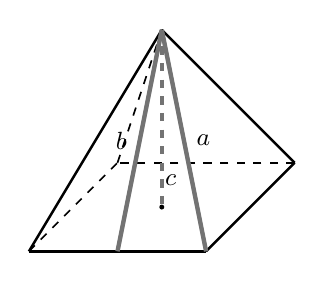
\begin{tikzpicture}[scale=0.75,font=\small,line join=round]\draw[line width=0.9pt] (0,0) -- (3,0);\draw[line width=0.9pt] (3,0) -- (4.5,1.5);\draw[dashed,line width=0.6pt] (4.5,1.5) -- (1.5,1.5);\draw[dashed,line width=0.6pt] (0,0) -- (1.5,1.5);\draw[line width=0.9pt] (3,0) -- (2.25,3.75);\draw[line width=0.9pt] (0,0) -- (2.25,3.75);\draw[line width=0.9pt] (4.5,1.5) -- (2.25,3.75);\draw[dashed,line width=0.6pt] (1.5,1.5) -- (2.25,3.75);\draw[line width=1.6pt,black!55] (2.25,3.75) -- (3,0);\draw[line width=1.6pt,black!55] (2.25,3.75) -- (1.5,0);\draw[line width=1.6pt,black!55,dashed] (2.25,3.75) -- (2.25,0.75);\fill (2.25,0.75) circle (1.2pt);\node[right] at (2.675,1.875) {$a$};\node[left] at (1.825,1.875) {$b$};\node[right,inner sep=1pt] at (2.25,1.2) {$c$};\end{tikzpicture}}{}{}
\medskip
\aufg{\hangindent7mm\hangafter1\nr{4.}Lisa zeichnet das Schrägbild eines Würfels mit $4$\,cm Kante auf ein Kärtchen. Welches Kärtchen ist das kleinste, auf das es passt? (Breite $\times$ Höhe)\par\smallskip\leftskip7mm \kreuz{$5$\,cm $\times$ $5$\,cm}\ \kreuz{$6$\,cm $\times$ $5$\,cm}\par\kreuz{$6$\,cm $\times$ $6$\,cm}\ \kreuz{$8$\,cm $\times$ $4$\,cm}}{}{{\scriptsize\color{mbgrau}Ziel\hspace{2mm}}}
\medskip
\par\vspace{3mm}\setlength{\kr}{\dimexpr\pagegoal-\pagetotal-10mm\relax}%
\ifdim\kr>12mm\karomerk{k}{D}\noindent{\scriptsize\color{mbgrau}Platz zum Rechnen}\par\nointerlineskip\vspace{1mm}\noindent
\begin{tikzpicture}\clip (0,0) rectangle ({\linewidth-0.5mm},\kr);\draw[black!16,line width=0.3pt,step=5mm] (0,0) grid (\linewidth,\kr);\end{tikzpicture}\fi\par
\clearpage\label{s:T}\noindent\colorbox{black!12}{\makebox[10mm]{\Large\bfseries\strut T}}\hspace{3mm}{\Large\bfseries Probetest}\par\smallskip
\noindent Gemischt wie in der Prüfung, ohne Beispiel. Etwa 20 Minuten.\par\medskip
\noindent\textbf{Aufgaben}\hspace{1em}{\small\color{mbgrau}\karohinweis{T}{Rechne unten im Karo.}{Rechne auf einem extra Blatt.} Vergleiche jede Aufgabe gleich mit dem Lösungsheft.}\par\smallskip
\aufg{\hangindent7mm\hangafter1\nr{1.}Wie viele Kanten hat eine Pyramide mit quadratischer Grundfläche?\par\smallskip\leftskip7mm \kreuz{$4$}\ \kreuz{$5$}\par\kreuz{$8$}\ \kreuz{$12$}}{}{}
\medskip
\aufgg{\hangindent7mm\hangafter1\nr{2.}Aus dem Netz im Bild wird ein Würfel gefaltet. Welche Fläche liegt C gegenüber?}{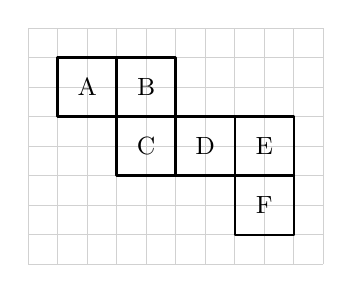
\begin{tikzpicture}[scale=0.75,font=\small,line join=round]\draw[black!18,line width=0.3pt,step=0.5] (-0.5,-0.5) grid (4.5,3.5);\draw[line width=0.9pt] (0,2) rectangle (1,3);\node at (0.5,2.5) {A};\draw[line width=0.9pt] (1,2) rectangle (2,3);\node at (1.5,2.5) {B};\draw[line width=0.9pt] (1,1) rectangle (2,2);\node at (1.5,1.5) {C};\draw[line width=0.9pt] (2,1) rectangle (3,2);\node at (2.5,1.5) {D};\draw[line width=0.9pt] (3,1) rectangle (4,2);\node at (3.5,1.5) {E};\draw[line width=0.9pt] (3,0) rectangle (4,1);\node at (3.5,0.5) {F};\end{tikzpicture}}{}{}
\medskip
\aufgg{\hangindent7mm\hangafter1\nr{3.}Aus dem Netz im Bild wird ein Körper gefaltet. Welcher Körper entsteht?\par\smallskip\leftskip7mm \kreuz{Dreiecksprisma}\ \kreuz{Pyramide mit dreieckiger Grundfläche}\par\kreuz{Pyramide mit quadratischer Grundfläche}}{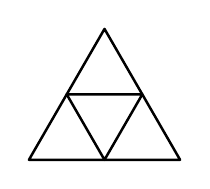
\begin{tikzpicture}[scale=0.6,font=\small,line join=round]\draw[line width=0.9pt] (0,0) -- (3.2,0) -- (1.6,2.771) -- cycle;\draw[line width=0.9pt] (1.6,0) -- (2.4,1.386) -- (0.8,1.386) -- cycle;\end{tikzpicture}}{}{}
\medskip
\aufgg{\hangindent7mm\hangafter1\nr{4.}Ein Quader ist $4$\,cm lang, $1$\,cm tief und $2$\,cm hoch. Zeichne sein Schrägbild in das Kästchenfeld.}{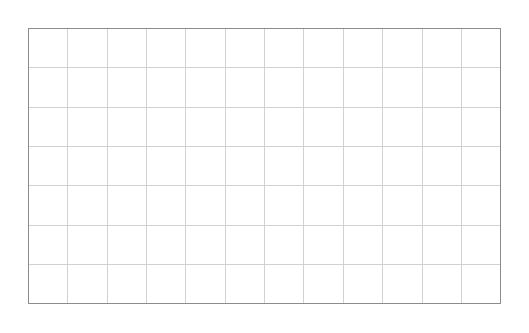
\begin{tikzpicture}[scale=1,font=\small,line join=round]\draw[black!18,line width=0.3pt,step=0.5] (0,0) grid (6,3.5);\draw[black!45,line width=0.4pt] (0,0) rectangle (6,3.5);\end{tikzpicture}}{}{}
\medskip
\aufg{\hangindent7mm\hangafter1\nr{5.}Aus einem Draht von $1$\,m Länge soll das Kantenmodell eines Würfels mit $8$\,cm Kantenlänge gebogen werden. Reicht der Draht?}{}{{\scriptsize\color{mbgrau}Ziel\hspace{2mm}}}
\medskip
\par\vspace{3mm}\setlength{\kr}{\dimexpr\pagegoal-\pagetotal-10mm\relax}%
\ifdim\kr>12mm\karomerk{k}{T}\noindent{\scriptsize\color{mbgrau}Platz zum Rechnen}\par\nointerlineskip\vspace{1mm}\noindent
\begin{tikzpicture}\clip (0,0) rectangle ({\linewidth-0.5mm},\kr);\draw[black!16,line width=0.3pt,step=5mm] (0,0) grid (\linewidth,\kr);\end{tikzpicture}\fi\par
\end{document}
